\documentclass[a4paper, 12pt]{article}

% packages
\usepackage{amssymb}
\usepackage[fleqn]{mathtools}
\usepackage{tikz}
\usepackage{enumerate}
\usepackage{bussproofs}
\usepackage{xcolor}
\usepackage[margin=1.3cm]{geometry}
\usepackage{logicproof}
\usepackage{diagbox}
\usepackage{listings}
\usepackage{graphicx}
\usepackage{lstautogobble}
\usepackage{hyperref}
\usepackage{multirow}
\usepackage{tipa}
\usepackage{pgfplots}

% tikz libraries
\usetikzlibrary{
    decorations.pathreplacing,
    arrows,
    shapes.gates.logic.US,
    circuits.logic.US,
    calc,
    automata,
    positioning,
    intersections
}

\pgfplotsset{compat=1.16}

\pgfmathdeclarefunction{gauss}{2}{%
  \pgfmathparse{1/(#2*sqrt(2*pi))*exp(-((x-#1)^2)/(2*#2^2))}%
}

\allowdisplaybreaks % allow environments to break
\setlength\parindent{0pt} % no indent

% shorthand for verbatim
% this clashes with logicproof, so maybe fix this at some point?
\catcode`~=\active
\def~#1~{\texttt{#1}}

% code listing
\lstdefinestyle{main}{
    numberstyle=\tiny,
    breaklines=true,
    showspaces=false,
    showstringspaces=false,
    tabsize=2,
    numbers=left,
    basicstyle=\ttfamily,
    columns=fixed,
    fontadjust=true,
    basewidth=0.5em,
    autogobble,
    xleftmargin=3.0ex,
    mathescape=true
}
\newcommand{\dollar}{\mbox{\textdollar}} %
\lstset{style=main}

% augmented matrix
\makeatletter
\renewcommand*\env@matrix[1][*\c@MaxMatrixCols c]{%
\hskip -\arraycolsep
\let\@ifnextchar\new@ifnextchar
\array{#1}}
\makeatother

% ceiling / floor
\DeclarePairedDelimiter{\ceil}{\lceil}{\rceil}
\DeclarePairedDelimiter{\floor}{\lfloor}{\rfloor}

% custom commands
\newcommand{\indefint}[2]{\int #1 \, \mathrm{d}#2}
\newcommand{\defint}[4]{\int_{#1}^{#2} #3 \, \mathrm{d}#4}
\newcommand{\pdif}[2]{\frac{\partial #1}{\partial #2}}
\newcommand{\dif}[2]{\frac{\mathrm{d}#1}{\mathrm{d}#2}}
\newcommand{\limit}[2]{\raisebox{0.5ex}{\scalebox{0.8}{$\displaystyle{\lim_{#1 \to #2}}$}}}
\newcommand{\limitsup}[2]{\raisebox{0.5ex}{\scalebox{0.8}{$\displaystyle{\limsup_{#1 \to #2}}$}}}
\newcommand{\summation}[2]{\sum\limits_{#1}^{#2}}
\newcommand{\product}[2]{\prod\limits_{#1}^{#2}}
\newcommand{\intbracket}[3]{\left[#3\right]_{#1}^{#2}}
\newcommand{\laplace}{\mathcal{L}}
\newcommand{\fourier}{\mathcal{F}}
\newcommand{\mat}[1]{\boldsymbol{#1}}
\renewcommand{\vec}[1]{\boldsymbol{#1}}
\newcommand{\rowt}[1]{\begin{bmatrix}
    #1
\end{bmatrix}^\top}
\DeclareMathOperator*{\argmax}{argmax}
\DeclareMathOperator*{\argmin}{argmin}

\newcommand{\lto}[0]{\leadsto\ }

\newcommand{\ulsmash}[1]{\underline{\smash{#1}}}

\newcommand{\powerset}[0]{\wp}
\renewcommand{\emptyset}[0]{\varnothing}

\makeatletter
\newsavebox{\@brx}
\newcommand{\llangle}[1][]{\savebox{\@brx}{\(\m@th{#1\langle}\)}%
  \mathopen{\copy\@brx\kern-0.5\wd\@brx\usebox{\@brx}}}
\newcommand{\rrangle}[1][]{\savebox{\@brx}{\(\m@th{#1\rangle}\)}%
  \mathclose{\copy\@brx\kern-0.5\wd\@brx\usebox{\@brx}}}
\makeatother
\newcommand{\lla}{\llangle}
\newcommand{\rra}{\rrangle}
\newcommand{\la}{\langle}
\newcommand{\ra}{\rangle}
\newcommand{\crnr}[1]{\text{\textopencorner} #1 \text{\textcorner}}
\newcommand{\bnfsep}[0]{\ |\ }
\newcommand{\concsep}[0]{\ ||\ }

\newcommand{\axiom}[1]{\AxiomC{#1}}
\newcommand{\unary}[1]{\UnaryInfC{#1}}
\newcommand{\binary}[1]{\BinaryInfC{#1}}
\newcommand{\trinary}[1]{\TrinaryInfC{#1}}
\newcommand{\quaternary}[1]{\QuaternaryInfC{#1}}
\newcommand{\quinary}[1]{\QuinaryInfC{#1}}
\newcommand{\dproof}[0]{\DisplayProof}

\newcommand{\ttbs}{\char`\\}
\newcommand{\lrbt}[0]{\ \bullet\ }

% colours
\newcommand{\violet}[1]{\textcolor{violet}{#1}}
\newcommand{\blue}[1]{\textcolor{blue}{#1}}
\newcommand{\red}[1]{\textcolor{red}{#1}}
\newcommand{\teal}[1]{\textcolor{teal}{#1}}

% reasoning proofs
\usepackage{ltablex}
\usepackage{environ}
\keepXColumns
\NewEnviron{reasoning}{
    \begin{tabularx}{\textwidth}{rlX}
        \BODY
    \end{tabularx}
}
\newcommand{\proofline}[3]{$(#1)$ & $#2$ & \hfill #3 \smallskip \\}
\newcommand{\proofarbitrary}[1]{& take arbitrary $#1$ \smallskip \\}
\newcommand{\prooftext}[1]{\multicolumn{3}{l}{#1} \smallskip \\}
\newcommand{\proofmath}[3]{$#1$ & = $#2$ & \hfill #3 \smallskip \\}
\newcommand{\prooftherefore}[1]{& $\therefore #1$ \smallskip \\}
\newcommand{\proofbc}[0]{\prooftext{\textbf{Base Case}}}
\newcommand{\proofis}[0]{\prooftext{\textbf{Inductive Step}}}

% ER diagrams
\newcommand{\nattribute}[4]{
    \node[draw, state, inner sep=0cm, minimum size=0.2cm, label=#3:{#4}] (#1) at (#2) {};
}
\newcommand{\mattribute}[4]{
    \node[draw, state, accepting, inner sep=0cm, minimum size=0.2cm, label=#3:{#4}] (#1) at (#2) {};
}
\newcommand{\dattribute}[4]{
    \node[draw, state, dashed, inner sep=0cm, minimum size=0.2cm, label=#3:{#4}] (#1) at (#2) {};
}
\newcommand{\entity}[3]{
    \node[] (#1-c) at (#2) {#3};
    \node[inner sep=0cm] (#1-l) at ($(#1-c) + (-1, 0)$) {};
    \node[inner sep=0cm] (#1-r) at ($(#1-c) + (1, 0)$) {};
    \node[inner sep=0cm] (#1-u) at ($(#1-c) + (0, 0.5)$) {};
    \node[inner sep=0cm] (#1-d) at ($(#1-c) + (0, -0.5)$) {};
    \draw
    ($(#1-c) + (-1, 0.5)$) -- ($(#1-c) + (1, 0.5)$) -- ($(#1-c) + (1, -0.5)$) -- ($(#1-c) + (-1, -0.5)$) -- cycle;
}
\newcommand{\relationship}[3]{
    \node[] (#1-c) at (#2) {#3};
    \node[inner sep=0cm] (#1-l) at ($(#1-c) + (-1, 0)$) {};
    \node[inner sep=0cm] (#1-r) at ($(#1-c) + (1, 0)$) {};
    \node[inner sep=0cm] (#1-u) at ($(#1-c) + (0, 1)$) {};
    \node[inner sep=0cm] (#1-d) at ($(#1-c) + (0, -1)$) {};
    \draw
    ($(#1-c) + (-1, 0)$) -- ($(#1-c) + (0, 1)$) -- ($(#1-c) + (1, 0)$) -- ($(#1-c) + (0, -1)$) -- cycle;
}

% AVL Trees
\newcommand{\avltri}[4]{
    \draw ($(#1)$) -- ($(#1) + #4*(0.5, -1)$) -- ($(#1) + #4*(-0.5, -1)$) -- cycle;
    \node at ($(#1) + #4*(0, -1) + (0, 0.5)$) {#3};
    \node at ($(#1) + #4*(0, -1) + (0, -0.5)$) {#2};
}

% RB Trees
\tikzset{rbtr/.style={inner sep=2pt, circle, draw=black, fill=red}}
\tikzset{rbtb/.style={inner sep=2pt, circle, draw=black, fill=black}}

% actual document
\begin{document}
    \section*{CO220 - Software Engineering Design}
        \subsection*{8th October 2019}
            \subsubsection*{Cost of Change}
                \begin{center}
                    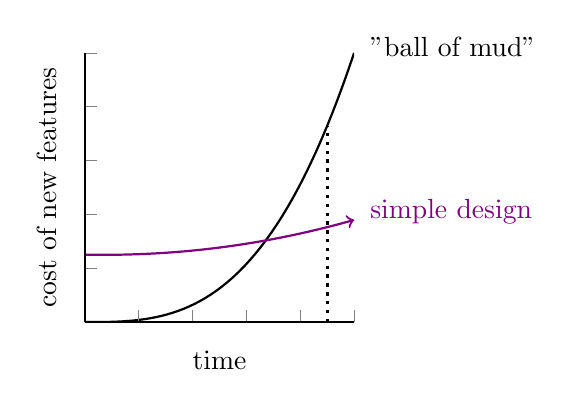
\begin{tikzpicture}
                        \begin{axis}[
                            axis on top=true,
                            axis line style=thick,
                            no markers, domain=0:10, samples=50,
                            axis lines*=left, xlabel={time}, ylabel={cost of new features},
                            height=5cm, width=5cm,
                            enlargelimits=false,
                            xticklabels={,,},
                            yticklabels={,,}
                        ]
                            \addplot[mark=none, black, very thick, dotted] coordinates {(9, 0) (9, 729)};
                            \addplot[thick] {\x^3};
                            \addplot[violet, thick, ->] {250+\x^1.75*ln(\x)};
                        \end{axis}
                        \node[anchor=west] at (3.5, 3.5) {"ball of mud"};
                        \node[anchor=west] at (3.5, 1.4) {\violet{simple design}};
                    \end{tikzpicture}
                \end{center}
                The "project heat death", denoted by the dotted line, is where the cost of adding new features outweighs the value gained by adding those features.
                Note that the initial cost of doing a simple design can be more expensive (since it requires more planning).
            \subsubsection*{Elements of Simple Design}
                This is arranged in a pyramid on the slides (since they "build up on each other") but I will write it as a list, starting from the bottom;
                \begin{enumerate}[1.]
                    \itemsep0em
                    \item \textbf{behaves correctly}
                        \medskip

                        It doesn't matter if the codebase is well structured, or the code is elegant if it doesn't do the right thing (is buggy, or isn't what the customer wanted).
                        \begin{itemize}
                            \itemsep0em
                            \item automated testing
                            \item test-driven development
                            \item mock objects
                        \end{itemize}
                    \item \textbf{minimises duplication}
                        \medskip

                        If something needs to be changed in the future, and it's in multiple places, it will have to be changed in all of those places which will take longer.
                        Additionally, it's also easy to miss, causing bugs.
                    \item \textbf{maximises clarity}
                        \medskip

                        Code should be easy to modify, such that the parts that need to be changed can be easily located.
                        Important especially if working with others.
                    \item \textbf{has fewer elements}
                        \medskip

                        Less important - we want to focus on the previous levels first, and don't want to lose the benefits by combining elements.
                \end{enumerate}
            \subsubsection*{Test-Driven Development / Behaviour Driven Development}
                Having a test suite provides confidence that the codebase still works, even after major changes.
                \begin{center}
                    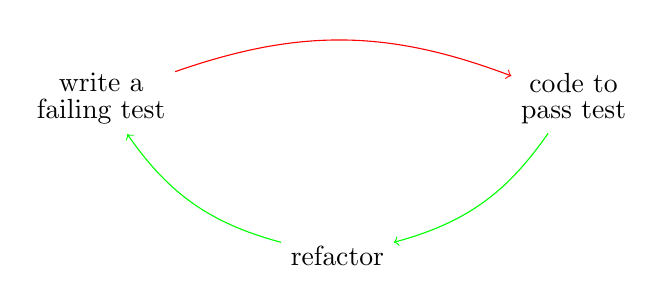
\begin{tikzpicture}[x=3cm]
                        \node (w) at (0, 0) {\shortstack{write a\\failing  test}};
                        \node (c) at (2, 0) {\shortstack{code to\\pass test}};
                        \node (r) at (1, -2) {refactor};
                        \draw
                        (w) edge[red, ->, bend left=20] (c)
                        (c) edge[green, ->, bend left=20] (r)
                        (r) edge[green, ->, bend left=20] (w);
                    \end{tikzpicture}
                \end{center}
                We start by writing failing tests, which seems counterintuitive, as there is no code to test.
                However, these tests are written as if the code was working - which gives us a specification on how the code \textbf{should} behave.
                We want to write code as quickly as possible that gets us from the \red{red} state (failing tests), to a \textcolor{green}{green} state (passing tests).
                This code is likely untidy - we can then tidy it up (which shouldn't break the tests).
                \medskip

                Additionally, it's not only about testing; we can replace the stages as follows;
                \begin{itemize}
                    \itemsep0em
                    \item API design \hfill (write a failing test)
                        \subitem "I wish there was a method that would take these parameters and do this"
                    \item internals design \hfill (code to pass test)
                        \subitem "Just making it work"
                    \item structural design \hfill (refactor)
                        \subitem "How can we improve the design?" (pyramid layers)
                \end{itemize}
                We focus more on what it should do (how it should behave), and not how it does it.
                For example, ~CustomerLookup~ should do the following;
                \begin{itemize}
                    \itemsep0em
                    \item finds customer by ID
                    \item fails for duplicate customers
                \end{itemize}
                The test is named as the expected result, and if it is true, then it behaves correctly.
                \begin{lstlisting}
                    public class CustomerLookupTest {
                      @Test
                      findsCustomerById() {
                        ...
                      }
                      @Test
                      failsForDuplicateCustomers() {
                        ...
                      }
                    }
                \end{lstlisting}
            \subsubsection*{Example of TDD}
                The object ~FibonacciSequence~ should do the following;
                \begin{itemize}
                    \itemsep0em
                    \item defines the first two terms to be one
                    \item has each term equal to the sum of the previous two
                    \item is not defined for negative terms
                \end{itemize}
                \begin{lstlisting}
                    ... // (FibonacciSequenceTest.java)

                    import static org.hamcrst.CoreMatchers.is;
                    import static org,junit.Assert.assertThat;

                    import org.junit.Test;

                    public class FibonacciSequenceTest {

                      @Test
                      public void definesFirstTwoTermsToBeOne() {
                        assertThat(new FibonacciSeqeunce().term(0), is(1));
                        assertThat(new FibonacciSeqeunce().term(1), is(1));
                      }
                    }
                \end{lstlisting}
                Obviously, none of this will work yet, as the code doesn't exist.
                However, we can use this to create the code as follows (this is incorrect, but our tests now pass);
                \begin{lstlisting}
                    ... // (FibonacciSequence.java)

                    public class FibonacciSequence {

                      public int term(int i) {
                        return 1;
                      }
                    }
                \end{lstlisting}
                We can then add more tests, which should now fail;
                \begin{lstlisting}
                    ... // (FibonacciSequenceTest.java)

                    public class FibonacciSequenceTest {
                      ...

                      @Test
                      public void hasEachTermTheSumOfPreviousTwo() {
                        assert(new FibonacciSeqeunce().term(2), is(2));
                        assert(new FibonacciSeqeunce().term(3), is(3));
                        assert(new FibonacciSeqeunce().term(4), is(5));
                      }
                    }
                \end{lstlisting}
                Similarly, we can modify the code again to add a naive implementation which performs it recursively;
                \begin{lstlisting}
                    ... // (FibonacciSequence.java)

                    public class FibonacciSequence {

                      public int term(int i) {
                        if (i < 2) {
                          return 1;
                        }
                        return term(i - 1) + term(i - 2);
                      }
                    }
                \end{lstlisting}
                Adding the last bullet point as a test;
                \begin{lstlisting}
                    ... // (FibonacciSequenceTest.java)

                    public class FibonacciSequenceTest {
                      ...

                      @Test
                      public void isNotDefinedForNegativeIndices() {
                        try {
                          new FibonacciSeqeunce().term(-1);
                          fail("should have thrown exception")
                        } catch (IllegalArgumentException iae) {
                          assertThat(iae.getMessage(), containsString("negative index"))
                        }
                      }
                    }
                \end{lstlisting}
                Fixing this, we add the following;
                \begin{lstlisting}
                    ... // (FibonacciSequence.java)

                    public class FibonacciSequence {

                      public int term(int i) {
                        if (i < 0) {
                          throw new IllegalArgumentException("negative index not supported");
                        }

                        ...
                      }
                    }
                \end{lstlisting}
                This is the only time I will actually write out every step, since that's the focus of TDD.
        \subsection*{11th October 2019}
            \subsubsection*{Feedback}
                Note that the names of the test files should be ~SomeObjectTest~, for ~SomeObject~.
                This convention allows the IDE to link the files, as well as having them in alphabetical order.
                Also always use a \textit{jUnit} library function;
                \begin{center}
                    ~assertThat(rul.size(), is(0))~ or ~assertEquals(0, rul.size())~

                    instead of

                    ~assert rul.size() == 0~
                \end{center}
                Generally make the LHS of fields the interface ~List~ instead of ~ArrayList~, and attempt to make it ~private~ and ~final~ (if possible).
                Additionally, any fields are reinitialised automatically by \textit{jUnit}, hence it doesn't need to be reset at the end of each test.
            \subsubsection*{Refactoring}
                This starts with multiple examples on handouts.
                As we're writing new code, we should look out for small changes that can improve the structure of our code.
                \medskip

                We can accumulate "technical debt" by writing code quickly to get a feature working, but we must fix it soon, otherwise it builds up leading to unhygienic code.
                \medskip

                Note that refactoring should be done with tools when possible (such as renaming identifiers), since the tool will be able to analyse the entire codebase to detect where changes need to be made.
                Behaviour should not be changed.
                \medskip

                The example after this is mostly using \textit{IntelliJ} tools wherever possible.
                One note to make is that sometimes it is helpful to get code into a state where it becomes similar enough to other parts of the code, to allow for the tool to do the work.
        \subsection*{15th October 2019}
            \subsubsection*{Sending Messages}
                Instead of considering how objects call methods, it may be beneficial to design how modules communicate with each other ("send messages").
                \medskip

                The idea is that when one object "sends a message", we don't really care how it does it, just that it performs the expected action.
            \subsubsection*{OOP}
                Typically, larger systems are built up of smaller units that work together.
                Some of these will be from the standard library, some of those will be written by us, and some others may be written by third parties.
                \begin{center}
                    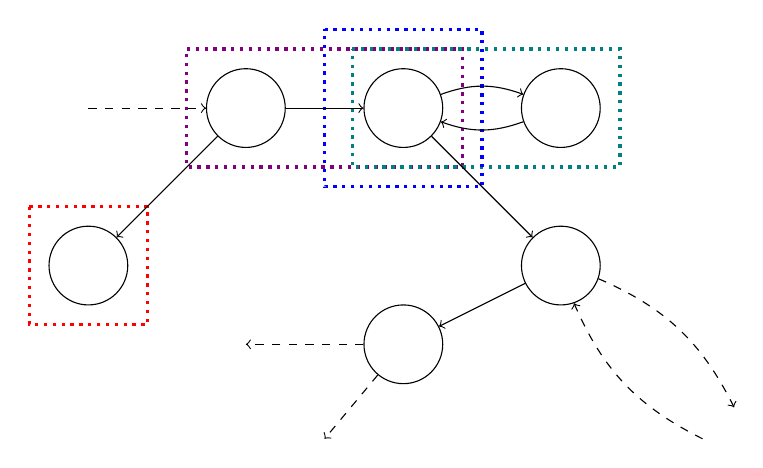
\begin{tikzpicture}[x=2cm, y=2cm]
                        \draw[violet, dotted, very thick] (-0.375, 0.375) -- (1.375, 0.375) -- (1.375, -0.375) -- (-0.375, -0.375) -- cycle;
                        \draw[teal, dotted, very thick] (0.675, 0.375) -- (2.375, 0.375) -- (2.375, -0.375) -- (0.675, -0.375) -- cycle;
                        \draw[red, dotted, very thick] (-1.375, -0.625) -- (-0.625, -0.625) -- (-0.625, -1.375) -- (-1.375, -1.375) -- cycle;
                        \draw[blue, dotted, very thick] (0.5, 0.5) -- (1.5, 0.5) -- (1.5, -0.5) -- (0.5, -0.5) -- cycle;
                        \node[state, minimum size=1cm] (a) at (0, 0) {};
                        \node[state, minimum size=1cm] (b) at (1, 0) {};
                        \node[state, minimum size=1cm] (c) at (2, 0) {};
                        \node[state, minimum size=1cm] (d) at (-1, -1) {};
                        \node[state, minimum size=1cm] (e) at (1, -1.5) {};
                        \node[state, minimum size=1cm] (f) at (2, -1) {};
                        \draw
                        (-1, 0) edge[->, dashed] (a)
                        (a) edge[->] (b)
                        (a) edge[->] (d)
                        (b) edge[->, bend left=20] (c)
                        (b) edge[->] (f)
                        (c) edge[->, bend left=20] (b)
                        (e) edge[->, dashed] (0, -1.5)
                        (e) edge[->, dashed] (0.5, -2.1)
                        (f) edge[->] (e)
                        (f) edge[->, dashed, bend left=20] (3.1, -1.9)
                        (2.9, -2.1) edge[->, dashed, bend left=20] (f);
                    \end{tikzpicture}
                \end{center}
                However, these components should be reusable, and they can be combined in a different way if needed (we can't really modify code in the standard library, etc).
                We want to have the possibility to swap out parts of the project without affecting other objects.
                The system shouldn't care how the object does a job, just that it does it.
                \begin{itemize}
                    \itemsep0em
                    \item \violet{\textbf{commands}} \hfill "please do $X$"
                        \medskip

                        This doesn't wait for a response, or a even a return value.
                    \item \teal{\textbf{queries}} \hfill "please tell me $Y$"
                        \medskip

                        Requests a bit of data, and then processes it.
                        If too many queries are used, we tend to have a central part of the process that deals with all the information which isn't flexible.
                        Ideally jobs are delegated to different components.
                    \item \red{\textbf{value objects}}
                        \medskip

                        These don't typically interact with other objects, and just holds some data and performs some computations.
                        These components can easily be tested.
                    \item \blue{\textbf{tell don't ask}}
                        \medskip

                        The role of this object is to coordinate other objects in the system.
                        Focusing on commands tends to give us more flexibility, but leads to different testing approaches.
                \end{itemize}
                Typically, asking looks like the following (can be characterised by a higher number of ~getX()~s);
                \begin{lstlisting}
                    table.getGrid().getColumnModel().getColumn(index).setPreferredWidth(newWidth);
                \end{lstlisting}
                Visually, the graph becomes something similar to this;
                \begin{center}
                    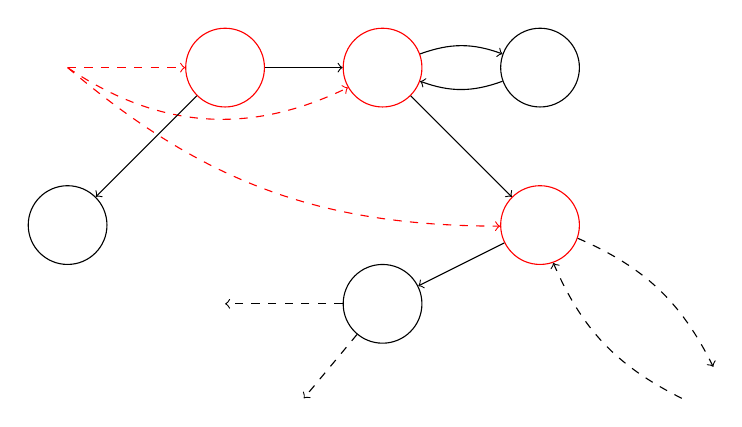
\begin{tikzpicture}[x=2cm, y=2cm]
                        \node[red, state, minimum size=1cm] (a) at (0, 0) {};
                        \node[red, state, minimum size=1cm] (b) at (1, 0) {};
                        \node[state, minimum size=1cm] (c) at (2, 0) {};
                        \node[state, minimum size=1cm] (d) at (-1, -1) {};
                        \node[state, minimum size=1cm] (e) at (1, -1.5) {};
                        \node[red, state, minimum size=1cm] (f) at (2, -1) {};
                        \draw
                        (-1, 0) edge[red, ->, dashed] (a)
                        (-1, 0) edge[red, ->, dashed, bend right=30] (b)
                        (-1, 0) edge[red, ->, dashed, bend right=20] (f)
                        (a) edge[->] (b)
                        (a) edge[->] (d)
                        (b) edge[->, bend left=20] (c)
                        (b) edge[->] (f)
                        (c) edge[->, bend left=20] (b)
                        (e) edge[->, dashed] (0, -1.5)
                        (e) edge[->, dashed] (0.5, -2.1)
                        (f) edge[->] (e)
                        (f) edge[->, dashed, bend left=20] (3.1, -1.9)
                        (2.9, -2.1) edge[->, dashed, bend left=20] (f);
                    \end{tikzpicture}
                \end{center}
            \subsubsection*{Testing Objects and Roles}
                When we want to test a given object, let it be $O$, we shouldn't have to implement the objects it depends on first.
                To do this, we use interfaces in Java to represent roles - which specifies what $O$ expects the other objects to do.
                An object may play different roles (hence implement multiple interfaces).
                \begin{center}
                    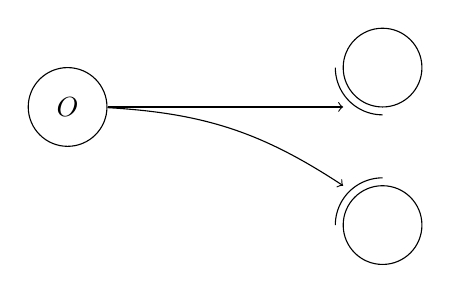
\begin{tikzpicture}
                        \node[state, minimum size=1cm] (a) at (0, 0.5) {$O$};
                        \node[state, minimum size=1cm] at (4, 1) {};
                        \node[state, minimum size=1cm] at (4, -1) {};
                        \draw[black, domain=180:270] plot ({4 + 0.6*cos(\x)}, {1 + 0.6*sin(\x)});
                        \draw[black, domain=90:180] plot ({4 + 0.6*cos(\x)}, {-1 + 0.6*sin(\x)});
                        \draw (a) edge[->, bend left=15] (3.5, -0.5);
                        \draw (a) edge[->] (3.5, 0.5);
                    \end{tikzpicture}
                \end{center}
                The object $O$ is the one we wish to test, and should be triggered by a call in the test suite.
            \subsubsection*{Mock Objects}
                To test objects that rely on stuff other objects that haven't been implemented yet (only an interface exists), we can use mock objects.
                \begin{center}
                    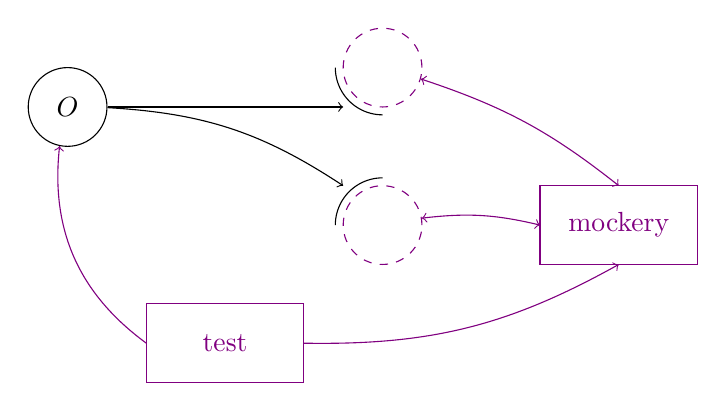
\begin{tikzpicture}
                        \node[state, minimum size=1cm] (a) at (0, 0.5) {$O$};
                        \node[violet, dashed, state, minimum size=1cm] (b) at (4, 1) {};
                        \node[violet, dashed, state, minimum size=1cm] (c) at (4, -1) {};
                        \draw[black, domain=180:270] plot ({4 + 0.6*cos(\x)}, {1 + 0.6*sin(\x)});
                        \draw[black, domain=90:180] plot ({4 + 0.6*cos(\x)}, {-1 + 0.6*sin(\x)});
                        \draw (a) edge[->, bend left=15] (3.5, -0.5);
                        \draw (a) edge[->] (3.5, 0.5);

                        \node[violet] at (2, -2.5) {test};
                        \draw[violet] (1, -2) -- (3, -2) -- (3, -3) -- (1, -3) -- cycle;
                        \draw[violet]
                        (1, -2.5) edge[->, bend left=30] (a)
                        (3, -2.5) edge[->, bend right=15] (7, -1.5)
                        (6, -1) edge[<->, bend right=10] (c)
                        (7, -0.5) edge[<->, bend right=10] (b);
                        \node[violet] at (7, -1) {mockery};
                        \draw[violet] (6, -0.5) -- (8, -0.5) -- (8, -1.5) -- (6, -1.5) -- cycle;
                    \end{tikzpicture}
                \end{center}
                When a test is run, we can test if $O$ sends messages to the mock objects.
                Instead of writing assertions about the state of $O$, we can write expectations for what should be called.
                \medskip

                An example is as follows (this is syntax from \textit{WebSequenceDiagrams}, because I don't want to draw it out);
                \begin{lstlisting}
                    Waiter->HeadChef: order(CHICKEN, APPLE)
                    HeadChef->PastryChef: order(APPLE)

                    Waiter->HeadChef: customerReadyFor(APPLE)
                    HeadChef->PastryChef: isCooked(APPLE)
                    PastryChef-->HeadChef: True
                    HeadChef->Waiter: serve(APPLE)

                    Waiter->HeadChef: customerReadyFor(APPLE)
                    HeadChef->PastryChef: isCooked(APPLE)
                    PastryChef-->HeadChef: False
                \end{lstlisting}
                In Java, we have the following for the tests;
                \begin{lstlisting}
                    ... // (HeadChefTest.java)

                    public class HeadChefTest {

                      @Rule
                      public JUnitRuleMockery context = new JUnitRuleMockery();

                      public final Order APPLE_TART = new Order("apple");
                      public final Order ROAST_CHICKEN = new Order("chicken");

                      Chef pastryChef = context.mock(Chef.class);
                      RestaurantWaiter waiter = context.mock(RestaurantWaiter.class);

                      @Test
                      public void delegatesDessertToPastryChef() {

                        HeadChef headChef = new HeadChef(pastryChef, waiter);

                        context.checking(new Expectations() {{
                          exactly(1).of(pastryChef).order(APPLE_TART);
                        }});

                        headChef.order(ROAST_CHICKEN, APPLE_TART);
                      }

                      @Test
                      public void asksWaiterToServeDessertIfCooked() {

                        HeadChef headChef = new HeadChef(pastryChef, waiter);

                        context.checking(new Expectations() {{
                          exactly(1).of(pastryChef).isCooked(APPLE_TART); will(returnValue(true));
                          exactly(1).of(waiter).serve(APPLE_TART);
                        }});

                        headChef.customerReadyFor(APPLE_TART);
                      }

                      @Test
                      public void doesNotAskWaiterToServeDessertIfNotCooked() {

                        HeadChef headChef = new HeadChef(pastryChef, waiter);

                        context.checking(new Expectations() {{
                          exactly(1).of(pastryChef).isCooked(APPLE_TART); will(returnValue(false));
                          never(waiter).serve(APPLE_TART);
                        }});

                        headChef.customerReadyFor(APPLE_TART);
                      }
                    }
                \end{lstlisting}
                Similarly for the ~HeadChef~;
                \begin{lstlisting}
                    ... // (HeadChef.java)

                    public class HeadChef {

                      private final Chef pastryChef;
                      private final RestaurantWaiter waiter;

                      public HeadChef(Chef pastryChef, RestaurantWaiter waiter) {
                        this.pastryChef = pastryChef;
                        this.waiter = waiter;
                      }

                      public void order(Order main, Order dessert) {
                        pastryChef.order(dessert);
                      }

                      public void customerReadyFor(Order dessert) {
                        if (pastryChef.isCooked(dessert)) {
                          waiter.serve(dessert);
                        }
                      }
                    }
                \end{lstlisting}
                Note that we have \textbf{interfaces} for ~Chef~ and ~RestaurantWaiter~, as they aren't implemented;
                \begin{lstlisting}
                    ... // (Chef.java)

                    public interface Chef {
                      void order(Order order);

                      bool isCooked(Order order);
                    }
                \end{lstlisting}
                \begin{lstlisting}
                    ... // (RestaurantWaiter.java)

                    public interface RestaurantWaiter {
                        void serve(Order order);
                    }
                \end{lstlisting}
        \subsection*{18th October 2019}
            \subsubsection*{Feedback}
                We only want to test each behaviour once, to avoid breaking tests elsewhere.
                Note that \textit{jMock} is more strict than \textit{Mockito}.
                Additionally, if we are expecting the same value in the behaviour, we don't have to make a new mock object if it won't be tested (hence we can just create a constant field).
                \begin{lstlisting}
                    ... // (CameraTest.java)

                    public class CameraTest {
                      ...

                      private static final byte[] PHOTO = new byte[8];
                      ...

                      @Test
                      public void switchingTheCameraOffPowersDownTheSensor() {

                        context.checking(new Expectations() {{
                          ignoring(sensor).powerUp();
                          exactly(1).of(sensor).powerDown();
                        }});

                        camera.powerOn();
                        camera.powerOff();
                      }

                      @Test
                      public void pressingTheShutterCopiesData() {

                        context.checking(new Expectations() {{
                          ignoring(sensor).powerUp();
                          exactly(1).of(sensor).readData(); will(returnValue(PHOTO));
                          exactly(1).of(memoryCard).write(PHOTO);
                        }});

                        camera.powerOn();
                        camera.pressShutter();
                      }
                    }
                \end{lstlisting}
            \subsubsection*{Designing for Flexibility}
                Bad design consists of the following properties;
                \begin{itemize}
                    \itemsep0em
                    \item \textbf{rigidity} \hfill difficult to change, possibly due to complex code (long methods, deep conditions etc.)
                    \item \textbf{fragility} \hfill making a change in one place could break another part of the code
                    \item \textbf{immobility} \hfill difficult to reuse code in another context
                \end{itemize}
            \subsubsection*{Law of Demeter}
                Recall the graph that had many ~getX()~s, the red lines reached across the graph, but the law of Demeter states that access should generally be to an object that is one "hop" away.
                This preserves flexibility.
                Violating this can cause fragility, as changing one part of the code could affect another part of the code that is far away.
                \medskip

                We can perform the following steps to extract a "trainwreck" into a method, which is then put into the next object down the "chain" of ~getX()~s.
                \begin{center}
                    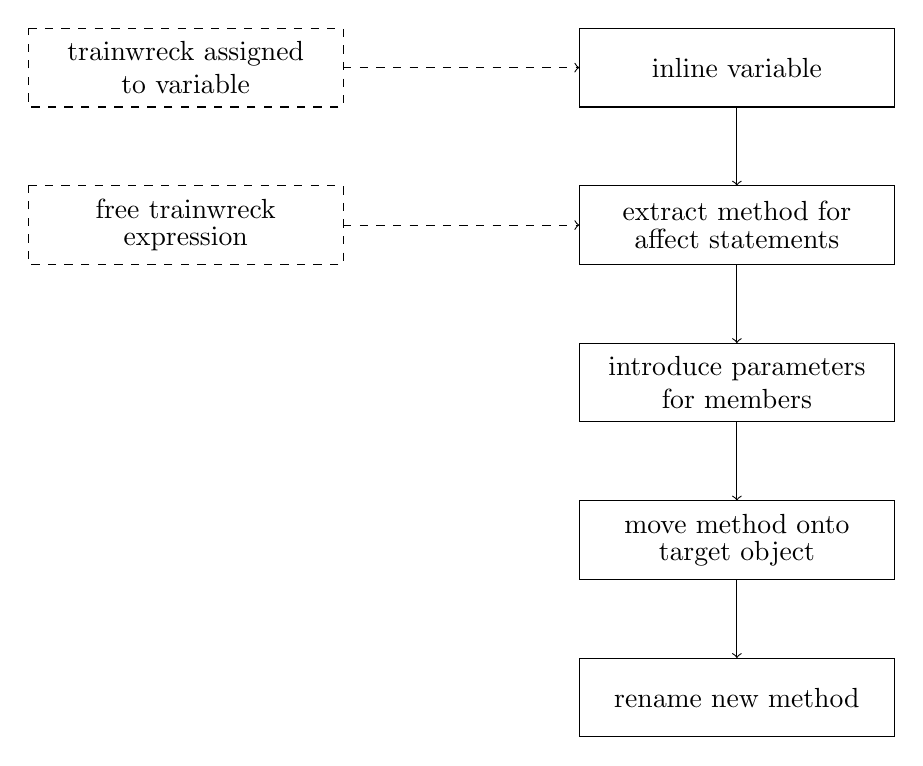
\begin{tikzpicture}
                        \draw
                        (4, -0.5) edge[->, dashed] (7, -0.5)
                        (4, -2.5) edge[->, dashed] (7, -2.5)
                        (9, -1) edge[->] (9, -2)
                        (9, -3) edge[->] (9, -4)
                        (9, -5) edge[->] (9, -6)
                        (9, -7) edge[->] (9, -8);
                        \begin{scope}[shift={(0, 0)}]
                            \node at (2, -0.5) {\shortstack{trainwreck assigned\\to variable}};
                            \draw[dashed] (0, 0) -- (4, 0) -- (4, -1) -- (0, -1) -- cycle;
                        \end{scope}
                        \begin{scope}[shift={(0, -2)}]
                            \node at (2, -0.5) {\shortstack{free trainwreck\\expression}};
                            \draw[dashed] (0, 0) -- (4, 0) -- (4, -1) -- (0, -1) -- cycle;
                        \end{scope}
                        \begin{scope}[shift={(7, 0)}]
                            \node at (2, -0.5) {inline variable};
                            \draw (0, 0) -- (4, 0) -- (4, -1) -- (0, -1) -- cycle;
                        \end{scope}
                        \begin{scope}[shift={(7, -2)}]
                            \node at (2, -0.5) {\shortstack{extract method for\\affect statements}};
                            \draw (0, 0) -- (4, 0) -- (4, -1) -- (0, -1) -- cycle;
                        \end{scope}
                        \begin{scope}[shift={(7, -4)}]
                            \node at (2, -0.5) {\shortstack{introduce parameters\\for members}};
                            \draw (0, 0) -- (4, 0) -- (4, -1) -- (0, -1) -- cycle;
                        \end{scope}
                        \begin{scope}[shift={(7, -6)}]
                            \node at (2, -0.5) {\shortstack{move method onto\\target object}};
                            \draw (0, 0) -- (4, 0) -- (4, -1) -- (0, -1) -- cycle;
                        \end{scope}
                        \begin{scope}[shift={(7, -8)}]
                            \node at (2, -0.5) {rename new method};
                            \draw (0, 0) -- (4, 0) -- (4, -1) -- (0, -1) -- cycle;
                        \end{scope}
                    \end{tikzpicture}
                \end{center}
            \subsubsection*{Defending against Null Pointer Exceptions}
                The following snippet of code has lines 3 and 5 added to protect against NPEs - however if this is needed frequently it could lead to code duplication;
                \begin{lstlisting}
                    void playTrack(String name) {
                      Track track = library.getTrack(name);
                      if (track != null) {
                        track.play();
                      }
                    }
                \end{lstlisting}
                Another approach is to have the \textbf{null object pattern}, which is an empty implementation;
                \begin{lstlisting}
                    interface Track {
                      public void play();
                    }

                    class NullTrack implements Track {
                      public void play() {
                        // do nothing
                      }
                    }
                \end{lstlisting}
                As a development team, it makes sense to agree on what will be done, whether it be using the null object pattern, or using Java's ~Optional~s.
            \subsubsection*{Coupling and Cohesion}
                \begin{itemize}
                    \itemsep0em
                    \item aim for \textbf{low coupling} between classes \hfill changing one part requires a change in the other
                    \item aim for \textbf{high cohesion} within each class \hfill a class should be specialised (less changes needed)
                \end{itemize}
                Ideally, we want to limit the "blast radius" of our changes, which is the amount of code we affect to just parts managed by us.
            \subsubsection*{Approaches}
                One extreme is to store all of the code in a single repository, allowing changes to be made when needed (given approval), which is done by Google.
                This has the benefit that a part can be changed in part of the code, and can also be fixed in another.
                However, due to the ability to affect other unrelated parts of the codebase, it can also lead to issues when updating a core object.
                \medskip

                The other extreme is to have modular code, which is individually versioned.
                That way, if something is updated, other modules can use older versions and update when needed (which doesn't break functionality straight away).
                However, updates will need to be done quite frequently, otherwise other modules will be behind.
                It's also difficult to make changes in other parts.
\end{document}
